% !TEX root = ../main.tex

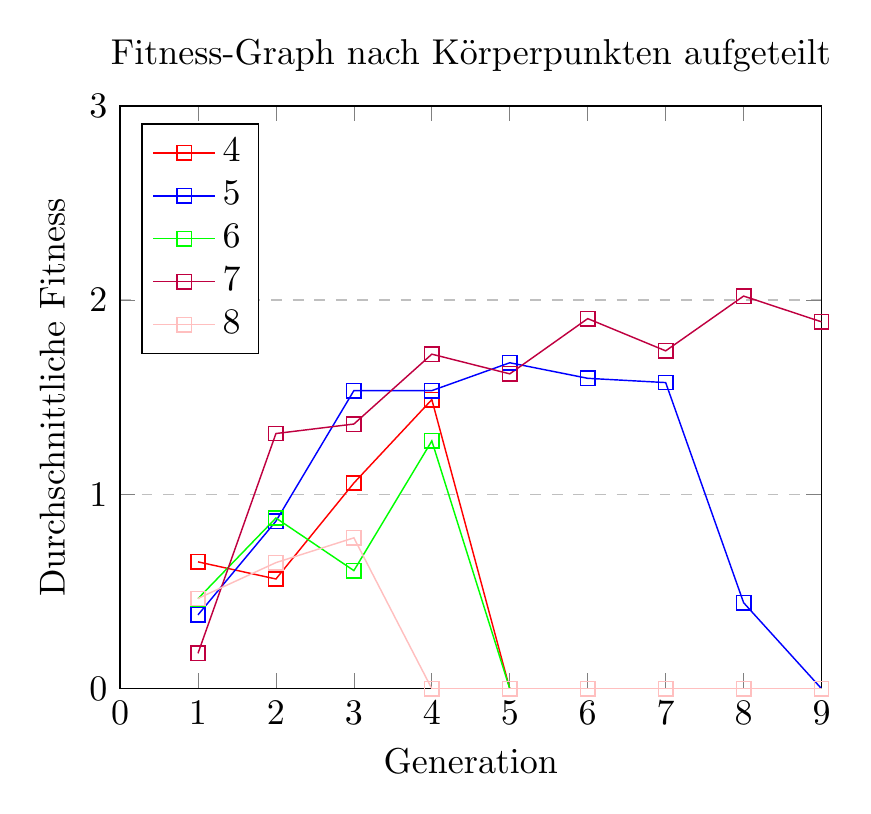
\begin{tikzpicture}[scale=1.3]
\begin{axis}[
    title={Fitness-Graph nach Körperpunkten aufgeteilt},
    xlabel={Generation},
    ylabel={Durchschnittliche Fitness},
    xmin=0, xmax=9,
    ymin=0, ymax=3,
    xtick={0,1,2,3,4,5,6,7,8,9},
    ytick={0,1,2,3},
    legend pos=north west,
    ymajorgrids=true,
    grid style=dashed,
]

\addplot[
    color=red,
    mark=square,
    ]
    coordinates {
		(1,0.6531646782329873)(2,0.5649720091810998)(3,1.0590192934741145)(4,1.4882885813713074)(5,0)(6,0)(7,0)(8,0)(9,0)
    };
    \addlegendentry{4}


\addplot[
    color=blue,
    mark=square,
    ]
    coordinates {
		(1,0.3802694280942281)(2,0.8626815751194954)(3,1.534655938545863)(4,1.534550075046718)(5,1.6780443640754503)(6,1.5979272299087965)(7,1.5759730805401448)(8,0.4428929388523102)(9,0)
    };
    \addlegendentry{5}


\addplot[
    color=green,
    mark=square,
    ]
    coordinates {
(1,0.46377276743833834)(2,0.878849039785564)(3,0.6080888311068217)(4,1.2757521867752075)(5,0)(6.0)(7,0)(8,0)(9,0)
    };
    \addlegendentry{6}

\addplot[
    color=purple,
    mark=square,
    ]
    coordinates {
		(1,0.1822953193138043)(2,1.3137148196498554)(3,1.362616437854189)(4,1.7222362977007162)(5,1.6208574524006019)(6,1.9052270071252304)(7,1.7392755072684056)(8,2.0213376003606567)(9,1.8886241616525998)
	};
    \addlegendentry{7}

\addplot[
    color=pink,
    mark=square,
    ]
    coordinates {
		(1,0.4648333308489426)(2,0.6492378941099894)(3,0.7767763224087263)(4,0)(5,0)(6,0)(7,0)(8,0)(9,0)
    };
    \addlegendentry{8}

\end{axis}
\end{tikzpicture}
